\documentclass[10pt,aspectratio=43]{beamer}
\usepackage{fontspec}
\IfFontExistsTF{arial.ttf}{\setsansfont{arial.ttf}[BoldFont=arialbd.ttf,ItalicFont=ariali.ttf,BoldItalicFont=arialbi.ttf]}{\setsansfont{TeX Gyre Heros}}
\IfFontExistsTF{consola.ttf}{\setmonofont{consola.ttf}}{\setmonofont{Latin Modern Mono}}
\usepackage{amsmath,amssymb,booktabs,graphicx,listings}
\usefonttheme{professionalfonts}
\definecolor{slideblue}{RGB}{73,69,181}
\definecolor{slidelight}{RGB}{170,168,220}
\setbeamercolor{structure}{fg=slideblue}
\setbeamercolor{frametitle}{fg=slideblue,bg=black!4}
\setbeamerfont{frametitle}{size=\Large}
\setbeamercolor{block title}{fg=white,bg=slideblue}
\setbeamercolor{block body}{fg=black,bg=black!3}
\setbeamertemplate{blocks}[rounded][shadow=true]
\setbeamertemplate{navigation symbols}{}
\setbeamersize{text margin left=5mm,text margin right=5mm}
\setbeamercolor{headleft}{fg=white,bg=slideblue}
\setbeamercolor{headright}{fg=black,bg=slidelight}
\setbeamertemplate{headline}{\leavevmode\hbox{%
\begin{beamercolorbox}[wd=.52\paperwidth,ht=2.8ex,dp=1.1ex,leftskip=2mm]{headleft}\tiny\insertsectionhead\end{beamercolorbox}%
\begin{beamercolorbox}[wd=.48\paperwidth,ht=2.8ex,dp=1.1ex,leftskip=2mm]{headright}\tiny\insertsubsectionhead\end{beamercolorbox}}}
\setbeamertemplate{footline}{\leavevmode\hbox{%
\begin{beamercolorbox}[wd=.34\paperwidth,ht=2.5ex,dp=1ex,center]{headleft}\tiny THỐNG KÊ TÍNH TOÁN\end{beamercolorbox}%
\begin{beamercolorbox}[wd=.43\paperwidth,ht=2.5ex,dp=1ex,center]{headright}\tiny C03107 -- Nhóm D -- Buổi 18\end{beamercolorbox}%
\begin{beamercolorbox}[wd=.23\paperwidth,ht=2.5ex,dp=1ex,center]{headleft}\tiny\ifnum\value{framenumber}>37 P\the\numexpr\value{framenumber}-37\relax\,/\,27\else\insertframenumber\,/\,37\fi\end{beamercolorbox}}}
\setbeamertemplate{frametitle}{\nointerlineskip\begin{beamercolorbox}[wd=\paperwidth,sep=1.5mm,leftskip=1mm]{frametitle}\begin{minipage}[c]{.82\paperwidth}\raggedright\insertframetitle\end{minipage}\hfill\raisebox{-1mm}{
\includegraphics[width=15mm]{assets/tdtu.png}}\end{beamercolorbox}}
\logo{}
\setbeamertemplate{itemize items}[triangle]
\setlength{\abovedisplayskip}{5pt}
\setlength{\belowdisplayskip}{5pt}
\newcommand{\src}[1]{\par\vfill} % Ẩn chú thích nguồn ở cuối mỗi slide; giữ khoảng cách bố cục.
\setlength{\emergencystretch}{1em}
\newcommand{\thn}{\hat\theta_n}
\newcommand{\ths}{\hat\theta_n^*}
\newcommand{\sestar}{\widehat{se}^{\,*}}
\newcommand{\Var}{\operatorname{Var}}
\newcommand{\Cov}{\operatorname{Cov}}
\newcommand{\normal}{\mathrm{Normal}}
\newcommand{\basic}{\mathrm{Basic}}
\lstset{language=R,basicstyle=\ttfamily\scriptsize,breaklines=true,columns=fullflexible,keepspaces=true,showstringspaces=false,keywordstyle=\color{black},frame=single,rulecolor=\color{black!15}}
\title{Khoảng tin cậy Bootstrap\\chuẩn tắc và cơ bản}
\subtitle{Cơ sở lý thuyết, xây dựng và đánh giá hiệu năng}
\author{Nhóm D}
\institute{Khoa Toán -- Thống kê\\Trường Đại học Tôn Đức Thắng\\Giảng viên hướng dẫn: ThS. Bùi Thùy Trang}
\date{Học kỳ 1, năm học 2026--2027}

% Giữ màu của bản gốc; nội dung bên dưới tiêu đề dùng nét thường.
\setbeamerfont{normal text}{series=\mdseries}
\setbeamerfont{block body}{series=\mdseries}
\setbeamerfont{itemize/enumerate body}{series=\mdseries}
\setbeamerfont{itemize/enumerate subbody}{series=\mdseries}
\setbeamerfont{alerted text}{series=\mdseries}
\setbeamercolor{alerted text}{fg=black}
\let\bfseries\mdseries
\definecolor{codegray}{gray}{0.15}
\begin{document}
\section{Mở đầu}
\subsection{Bài toán và nội dung}
\begin{frame}{Buổi 18: Normal CI và Basic CI}
\titlepage
\src{Báo cáo Nhóm D, trang bìa.}
\end{frame}
\begin{frame}{Mục lục}
\begin{enumerate}
\setlength{\itemsep}{.35em}
\item Tổng quan và bối cảnh nghiên cứu
\item Phân phối thực nghiệm và lấy mẫu lại
\item Xây dựng khoảng tin cậy Normal và Basic
\item So sánh Normal và Basic
\item Hai ví dụ tính toán Bootstrap
\item Mô phỏng Monte Carlo bằng R
\item Ứng dụng khoảng tin cậy trong y sinh
\item Percentile và tính bất biến khi đổi thang
\item Kết luận và khuyến nghị
\end{enumerate}
\end{frame}

\begin{frame}{Liên hệ với các chương đã học}
\begin{enumerate}
\item Chương 1 phát sinh các giá trị $X_1,\ldots,X_N$ từ một phân phối đã biết.
\item Chương 2 dùng trung bình Monte Carlo để xấp xỉ kỳ vọng.
\[
  E[f(X)]\approx \frac{1}{N}\sum_{j=1}^{N} f(X_j).
\]
\item Chương 3 mô phỏng các mẫu để đánh giá ước lượng, chẳng hạn $\bar X$ dùng cho $\mu$.
\item Chương 4 lấy mẫu lại từ phân phối thực nghiệm để xây dựng khoảng tin cậy.
\end{enumerate}
\textit{Trong bài này dùng $n$ cho cỡ mẫu, $B$ cho số lần lấy lại, $K$ cho số lần mô phỏng mẫu gốc.}
\src{main.tex, mục 1, 2.3 và 6.1. Rizzo (2019), tr. 147--148, 213--215.}
\end{frame}

\begin{frame}{Bài toán: từ ước lượng điểm đến khoảng}
\[
X_1,\ldots,X_n\overset{\mathrm{i.i.d.}}\sim F,\quad
\theta=\theta(F),\quad \thn=\thn(X_1,\ldots,X_n).
\]
Một thủ tục khoảng cho hai cận ngẫu nhiên $L(X),U(X)$.
\[CP_F=P_F\{L(X)\le\theta(F)\le U(X)\}.\]
\begin{block}{Mức danh nghĩa và mức thực}
$1-\alpha=0{,}95$ là mục tiêu thiết kế. Giá trị $CP_F$ thực tế có thể khác 0,95 do cỡ mẫu và chất lượng xấp xỉ.
\end{block}
Sau khi quan sát mẫu, hai cận đã cố định; xác suất bao phủ xét trên quá trình lặp lại lấy mẫu.
\src{Báo cáo, mục 1.1, 3.1 và 6.1; Chương 4, slide 55.}
\end{frame}

\begin{frame}{Hai phân phối và hai quy mô tính toán}
\begin{itemize}
\item $F$: tổng thể chưa biết trong bài toán thực tế.
\item $F_n^*$: phân phối thực nghiệm xác định từ mẫu gốc.
\item $n$: số quan sát gốc, quyết định thông tin về $F$.
\item $B$: số lần lấy mẫu Bootstrap từ một $F_n^*$ cố định.
\item $K$: số mẫu gốc trong thí nghiệm Monte Carlo đánh giá phương pháp.
\end{itemize}
\begin{block}{Phân biệt}
Tăng $B$ làm phép tính Bootstrap ổn định hơn. Tăng $K$ làm đánh giá coverage ổn định hơn. Cả hai không thay thế việc tăng $n$.
\end{block}
\src{Báo cáo, mục 2.3 và 6.1.}
\end{frame}

\section{Cơ sở Bootstrap}
\subsection{Ký hiệu và phân phối thực nghiệm}
\begin{frame}{Quy ước ký hiệu}
\small
\begin{tabular}{lp{8.7cm}}\toprule
$F_n^*=F_x^*$ & Báo cáo dùng $F_n^*$; slide cô dùng $F_x^*$ khi giữ cố định mẫu $x$.\\[1mm]
$\thn$ & Thống kê trên mẫu gốc; $\hat\theta_n^{*(b)}$ trên mẫu lấy lại thứ $b$.\\[1mm]
$P^*,E^*,\Var^*$ & Có điều kiện theo mẫu gốc $x$.\\[1mm]
$\overline{\hat\theta_n^*}$ & Trung bình của $B$ giá trị thống kê Bootstrap.\\[1mm]
$\hat\theta^*_{n,(r)}$ & Giá trị thứ $r$ sau sắp xếp, khác chỉ số lặp $(b)$.\\[1mm]
$q_p^*$ & Phân vị mức $p$; nêu rõ type và tính chính xác hay mô phỏng.\\[1mm]
$z_{1-\alpha/2}$ & $\Phi^{-1}(1-\alpha/2)>0$; slide cô gọi cùng số này là $z_{\alpha/2}$.\\\bottomrule
\end{tabular}
\src{Báo cáo, mục 2--3, 6; Chương 4, slide 9, 29, 53, 58.}
\end{frame}

\begin{frame}{Phân phối thực nghiệm}
Cho mẫu quan sát $x=(x_1,\ldots,x_n)$. Chọn chỉ số $J$ đều trên $\{1,\ldots,n\}$ và đặt $X^*=x_J$.
\[
F_n^*(t)=P^*(X^*\le t)
=\frac{1}{n}\sum_{i=1}^{n}\mathrm{I}_{(-\infty,t]}(x_i).
\]
\[
P(J=i)=\frac1n,\qquad
P^*(X^*=a)=\frac{\#\{i:x_i=a\}}{n}.
\]
Với $x=(1,1,1,9)$, ba vị trí mang giá trị $1$ nên $P^*(X^*=1)=3/4$. Tại $t=8$, $F_n^*(8)=3/4$.
\src{main.tex, mục 2.1 và 2.3. Rizzo (2019), tr. 213--214.}
\end{frame}

\begin{frame}{Hai moment của ECDF}
Trước khi quan sát mẫu, với $t$ cố định, đặt $Y_i=\mathrm{I}_{\{X_i\le t\}}$.
\[
Y_i\sim\operatorname{Bernoulli}(F(t)),\qquad
nF_n^*(t)=\sum_{i=1}^nY_i\sim\operatorname{Binomial}(n,F(t)).
\]
Từ kỳ vọng và phương sai của tổng các biến độc lập:
\[
E[F_n^*(t)]=F(t),\qquad
\Var[F_n^*(t)]=\frac{F(t)[1-F(t)]}{n}.
\]
\textit{Khi $n$ tăng, luật số lớn cho hội tụ tại mỗi $t$ cố định.}
\src{main.tex, mục 2.1. Lập luận trực tiếp từ chỉ thị Bernoulli.}

\par\small\hyperlink{r1}{\textit{Mô phỏng ECDF và chồng lên CDF chuẩn (R1)}}
\end{frame}

\begin{frame}{Plug-in và moment thực nghiệm}
Thay $F$ chưa biết bằng $F_n^*$ trong $\theta(F)$ để được $\thn=\theta(F_n^*)$.
\begin{align*}
E^*(X^*)&=\sum_{i=1}^n x_iP(J=i)=\frac{1}{n}\sum_{i=1}^n x_i=\bar x,\\
\Var^*(X^*)&=\frac{1}{n}\sum_{i=1}^n(x_i-\bar x)^2.
\end{align*}
Hai công thức cộng theo \textit{vị trí}. Với $x=(1,1,1,9)$, cũng có thể gộp theo giá trị và tính $1(3/4)+9(1/4)=3$.
\src{main.tex, mục 2.2. Rizzo (2019), tr. 213--215.}
\end{frame}

\section{Cơ sở Bootstrap}
\subsection{Lấy mẫu lại và sai số chuẩn}
\begin{frame}{Bootstrap SE: độ phân tán của thống kê}
Lấy độc lập $B$ mẫu có hoàn lại, mỗi mẫu cỡ $n$, từ $F_n^*$.
\[
\hat\theta_n^{*(b)}=\thn(X_1^{*(b)},\ldots,X_n^{*(b)}),\qquad
\overline{\hat\theta_n^*}=\frac1B\sum_{b=1}^B\hat\theta_n^{*(b)}.
\]
\begin{block}{Ước lượng Monte Carlo của $se^*(\thn)=\sqrt{\Var^*(\ths)}$}
\[\sestar(\thn)=\sqrt{\frac1{B-1}\sum_{b=1}^B
 (\hat\theta_n^{*(b)}-\overline{\hat\theta_n^*})^2}.\]
\end{block}
Mẫu số $B-1$ hiệu chỉnh phương sai; không chia thêm $\sqrt B$ vì cần độ lệch chuẩn của thống kê, không phải của trung bình mô phỏng.
\src{Báo cáo, thuật toán 2.1 và (2.12); Chương 4, slide 27--29.}
\end{frame}

\begin{frame}{Tăng số lần lấy lại giúp được điều gì?}
Giữ cố định dữ liệu $x$. Nếu $E^*[(\ths)^2]<\infty$ thì
\[\sestar(\thn)\xrightarrow[B\to\infty]{\mathrm{a.s.}}se^*(\thn).\]
\begin{enumerate}
\item Thay $F$ bằng $F_n^*$: cần dữ liệu đủ thông tin và phương pháp hợp lệ với thống kê đang xét.
\item Tính đặc trưng dưới $F_n^*$ bằng $B$ lần lấy lại: cần đủ độ chính xác Monte Carlo.
\end{enumerate}
Tăng $B$ chủ yếu cải thiện bước 2. Nó không tự làm $se^*(\thn)$ bằng sai số chuẩn thật.
\src{Báo cáo, mục 2.3; chứng minh bằng moment mẫu ở phụ lục.}
\end{frame}

\section{Khoảng tin cậy Bootstrap}
\subsection{Normal CI}
\begin{frame}{Normal CI: từ chuẩn hóa đến hai cận}
Nếu $\operatorname{bias}(\thn)$ nhỏ so với SE và xấp xỉ chuẩn hợp lý:
\[Z=\frac{\thn-\theta}{se(\thn)}\approx N(0,1).\]
Với $z=z_{1-\alpha/2}$, $P(-z\le Z\le z)\approx1-\alpha$.
\[-z\,se(\thn)\le\thn-\theta\le z\,se(\thn)\]
\[\Longleftrightarrow\quad\thn-z\,se(\thn)\le\theta\le\thn+z\,se(\thn).\]
\begin{block}{Thay SE bằng Bootstrap SE}
\[CI_{\normal}=\left[\thn-z\sestar(\thn),\;\thn+z\sestar(\thn)\right].\]
\end{block}
\src{Báo cáo, (3.1)--(3.2); Chương 4, slide 52--54. Tâm khoảng theo thống kê gốc.}
\end{frame}

\begin{frame}{Điều kiện của Normal CI}
\begin{itemize}
\item Cần xấp xỉ chuẩn của thống kê; dữ liệu gốc không bắt buộc chuẩn.
\item Cần bias đủ nhỏ ở thang SE; chuẩn hóa quanh $E(\thn)$ chưa tự cho chuẩn hóa quanh $\theta$.
\item Cần Bootstrap SE phản ánh hợp lý mức dao động thật.
\item Khoảng đối xứng quanh $\thn$ có thể kém với mẫu nhỏ, phân phối lệch hoặc tham số sát biên.
\end{itemize}
\[\frac{\thn-\theta}{se(\thn)}=
\frac{\thn-E(\thn)}{se(\thn)}+
\frac{E(\thn)-\theta}{se(\thn)}.\]
Số hạng cuối cho thấy vì sao điều kiện bias quan trọng.
\src{Báo cáo, mục 3.1.1, 4.2.1; Chương 4, slide 52--53.}
\end{frame}

\section{Khoảng tin cậy Bootstrap}
\subsection{Basic CI}
\begin{frame}{Basic CI: xấp xỉ phân phối sai số}
Đặt $\delta=\thn-\theta$, $\delta^*=\ths-\thn$.
\begin{block}{Bước thống kê}
Phân phối có điều kiện của sai số Bootstrap cần xấp xỉ phân phối sai số lấy mẫu, ở thang đo thích hợp.
\end{block}
Giữ $x$ cố định, $\thn$ là hằng số nên
\[q_p^*(\delta^*)=q_p^*(\ths)-\thn=q_p^*-\thn.\]
Đặt $l=q_{\alpha/2}^*-\thn$, $u=q_{1-\alpha/2}^*-\thn$.
\[P_F\{l\le\thn-\theta\le u\}\approx1-\alpha.\]
Ở phân phối rời rạc, hai phân vị không nhất thiết kẹp đúng $1-\alpha$ khối xác suất.
\src{Báo cáo, mục 3.2.1, (3.3)--(3.6); Chương 4, slide 56--58.}
\end{frame}

\begin{frame}{Basic CI: đảo bất đẳng thức}
Với $l=q_{\alpha/2}^*-\thn$, $u=q_{1-\alpha/2}^*-\thn$:
\begin{align*}
l\le\thn-\theta\le u
&\Longleftrightarrow l-\thn\le-\theta\le u-\thn\\
&\Longleftrightarrow\thn-u\le\theta\le\thn-l.
\end{align*}
\begin{block}{Khoảng Basic}
\[CI_{\basic}=\left[2\thn-q_{1-\alpha/2}^*,\;2\thn-q_{\alpha/2}^*\right].\]
\end{block}
Phân vị lớn tạo cận dưới vì khi nhân với $-1$ phải đảo chiều.
\alert{Đại số trên đúng chính xác; coverage xấp xỉ phụ thuộc bước xấp xỉ phân phối sai số.}
\src{Báo cáo, Định lý 3.1 và (3.7); Chương 4, slide 57--58.}
\end{frame}

\begin{frame}{Thuật toán lấy mẫu lại}
\begin{enumerate}
\item Tính $\thn=t(x)$ trên mẫu gốc $x=(x_1,\ldots,x_n)$.
\item Với mỗi $b=1,\ldots,B$, chọn độc lập $n$ chỉ số $J_{b,1},\ldots,J_{b,n}$ đều trên $\{1,\ldots,n\}$.
\item Tạo $x^{*(b)}=(x_{J_{b,1}},\ldots,x_{J_{b,n}})$ và tính $\hat\theta_n^{*(b)}=t(x^{*(b)})$.
\item Tính SE và hai phân vị từ $B$ giá trị thống kê, rồi thế vào hai công thức cận.
\end{enumerate}
\textit{Ví dụ liệt kê dùng type 1. Mô phỏng đánh giá coverage dùng type 7.}
\src{main.tex, thuật toán ở mục 2.3 và 3.3. Rizzo (2019), tr. 213--215, 225--226.}
\end{frame}

\section{So sánh phương pháp}
\subsection{Normal và Basic}
\begin{frame}{Normal CI và Basic CI}
\small\renewcommand{\arraystretch}{1.4}
\begin{tabular}{p{2.2cm}p{4.1cm}p{4.1cm}}\toprule
Tiêu chí & Normal & Basic\\\midrule
Cơ sở & Xấp xỉ chuẩn quanh tham số & Xấp xỉ phân phối sai số\\
Đầu vào & Thống kê gốc và Bootstrap SE & Thống kê gốc và hai phân vị\\
Hình dạng & Đối xứng quanh $\thn$ & Có thể bất đối xứng\\
Độ chệch & Không hiệu chỉnh trong phiên bản này & Phản chiếu phân vị, không bảo đảm loại bỏ bias\\
Hiệu năng & Cần kiểm tra coverage & Cần kiểm tra coverage\\\bottomrule
\end{tabular}
\src{Báo cáo, bảng 4.1.}
\end{frame}
\begin{frame}{Trung bình và phương sai mẫu}
Trong hai ví dụ và mô phỏng, tham số quan tâm là $\mu$. Thống kê dùng để ước lượng là
\[
\bar X=\frac1n\sum_{i=1}^n X_i,\qquad
S^2=\frac1{n-1}\sum_{i=1}^n(X_i-\bar X)^2.
\]
Nếu $X_i$ độc lập và cùng phân phối $N(\mu,\sigma^2)$, tổng các biến chuẩn vẫn là biến chuẩn. Vì vậy:
\[
\bar X\sim N\left(\mu,\frac{\sigma^2}{n}\right).
\]
Mỗi mẫu lấy lại cho một giá trị $\bar X^*$. Phân phối các giá trị này dùng để dựng khoảng cho $\mu$.
\src{main.tex, mục 5--6. Rizzo (2019), tr. 224--225. Ghi chú Google Docs.}
\end{frame}
\section{Ví dụ}
\subsection{Liệt kê phân phối Bootstrap}
\begin{frame}{Ví dụ 1: mẫu đối xứng}
\[x=(1,2,3),\qquad\thn=2,\qquad n^n=3^3=27.\]
\small\begin{tabular}{c*{7}{c}}\toprule
$\bar X^*$ & $1$ & $4/3$ & $5/3$ & $2$ & $7/3$ & $8/3$ & $3$\\
Tần số &1&3&6&7&6&3&1\\\bottomrule
\end{tabular}
\[se^*(\bar X)=\sqrt{2/9}\approx0.4714,\quad q_{.025}^*=1,\quad q_{.975}^*=3.\]
\[CI_{\normal}\approx [1.076,\,2.924],\qquad CI_{\basic}=[1.000,\,3.000].\]
Mỗi bộ chỉ số có xác suất $1/27$. Bảng tần số cho phân phối có điều kiện của $\bar X^*$.
\src{Báo cáo, mục 5.1 và bảng 5.1.}
\end{frame}
\begin{frame}{Ví dụ 2: mẫu lệch phải}
\[x=(1,1,1,9),\qquad\thn=3,\qquad4^4=256.\]
\small\begin{tabular}{c*{5}{c}}\toprule
$\bar X^*$&1&3&5&7&9\\
Tần số&81&108&54&12&1\\\bottomrule
\end{tabular}
\[se^*=\sqrt3\approx1.7321,\quad q_{.025}^*=1,\quad q_{.975}^*=7.\]
\[CI_{\normal}\approx [-0.395,\,6.395],\qquad CI_{\basic}=[-1.000,\,5.000].\]
$M\sim\mathrm{Binomial}(4,1/4)$, $\bar X^*=1+2M$. Vì vậy $se^*=\sqrt{4\Var(M)}=\sqrt3$.
\src{Báo cáo, mục 5.2.}
\end{frame}
\begin{frame}{Phân phối Bootstrap của hai ví dụ}
\centering
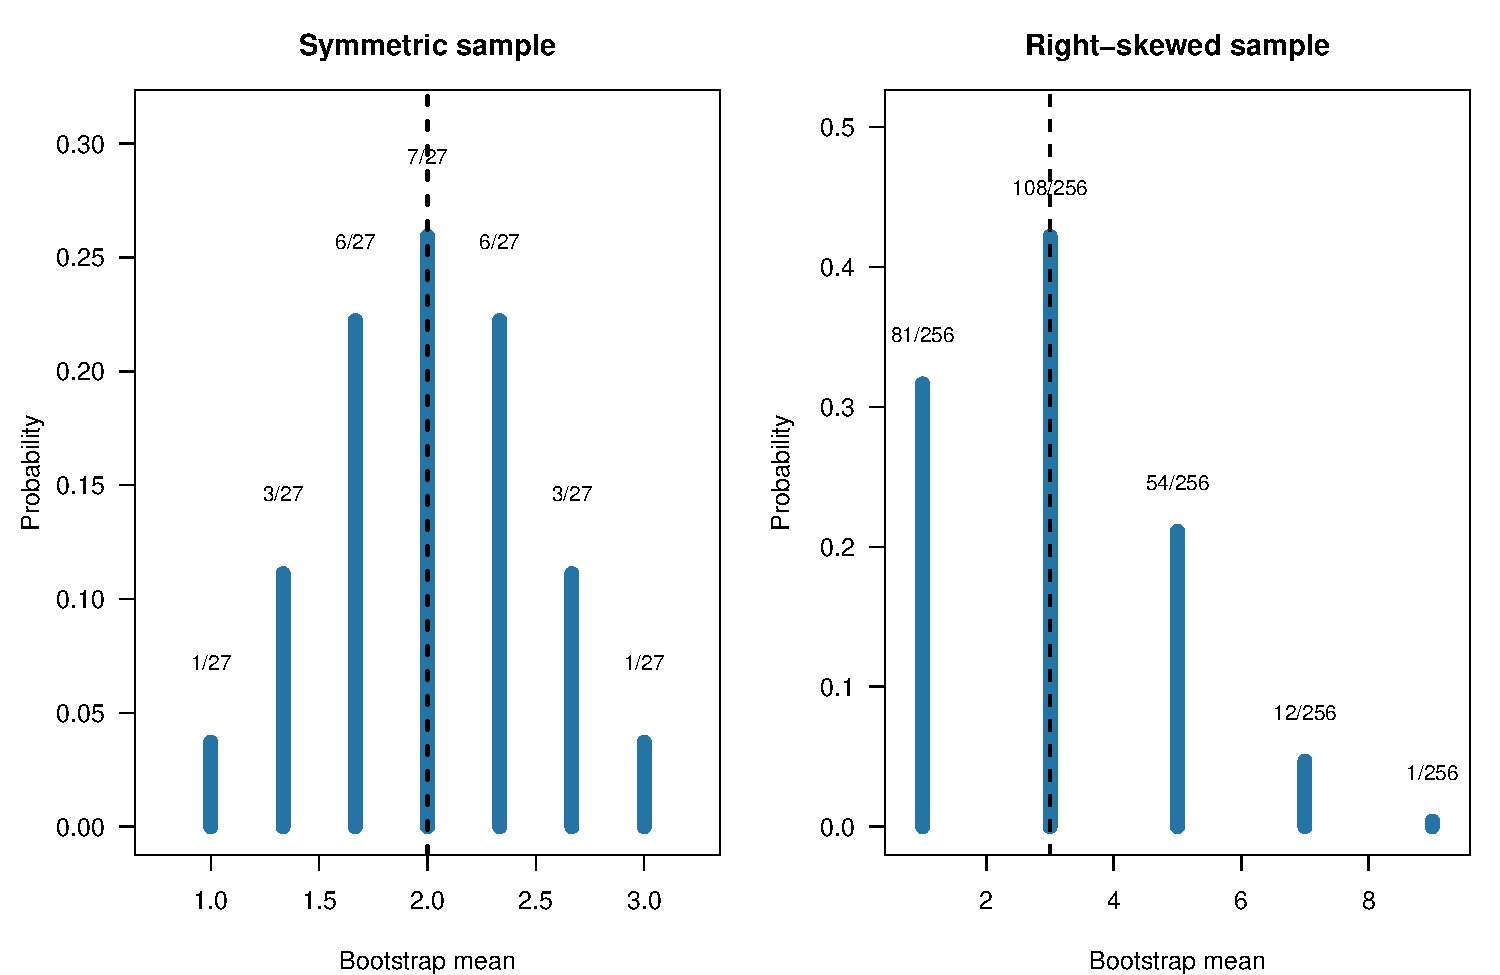
\includegraphics[width=.93\textwidth,height=.65\textheight,keepaspectratio]{assets/example-bootstrap-distributions.pdf}
\par\small Trục ngang là $\bar X^*$. Chiều cao là tần số chia cho số bộ chỉ số. Đường đứt đánh dấu $\bar x$.
\src{Báo cáo, hình 5.1; mã R nhóm D.}
\par\small\hyperlink{r2}{\textit{Liệt kê bộ chỉ số và đếm tần số (R2)}}
\end{frame}
\section{Mô phỏng Monte Carlo}
\subsection{Hai vòng và hiệu năng}
\begin{frame}{Thiết kế mô phỏng: hai vòng lặp}
\begin{itemize}
\item Tham số trong mô phỏng là trung bình tổng thể $\theta=\mu$.
\item Bốn kịch bản: $N(0,1)$ và $\operatorname{Exp}(1)$, mỗi phân phối có $n=12,40$.
\item Vòng ngoài: $K=10000$ mẫu độc lập từ tổng thể đã chọn.
\item Vòng trong: $B=1999$ mẫu Bootstrap cho mỗi mẫu gốc.
\item Mức danh nghĩa 95\%, seed 20260925, phân vị type 7.
\end{itemize}
\begin{block}{Trình tự}
Sinh mẫu gốc, tạo Bootstrap, tính các khoảng, ghi nhận có chứa tham số thật và ghi độ dài.
\end{block}
\src{main.tex, mục 6.1. Rizzo (2019), tr. 188--189 và Project 8.A, tr. 241.}
\end{frame}
\begin{frame}{Coverage và độ dài trung bình}
Với khoảng $[L_k,U_k]$ ở lần lặp ngoài thứ $k$:
\[\widehat{CP}=\frac1K\sum_{k=1}^K\mathrm{I}_{\{L_k\le\theta\le U_k\}},\]
\[\widehat{AL}=\frac1K\sum_{k=1}^K(U_k-L_k),\]
\[\widehat{MCSE}(\widehat{CP})=\sqrt{\frac{\widehat{CP}(1-\widehat{CP})}{K}}.\]
\begin{itemize}
\item Coverage cần gần mức danh nghĩa.
\item Khoảng ngắn cần được xét cùng mức bao phủ.
\end{itemize}
\src{Báo cáo, mục 6.1; liên hệ Chương 3, slide 22.}
\end{frame}
\begin{frame}[fragile]{Mã R dựng khoảng trên một mẫu}
\begin{lstlisting}
means <- colMeans(matrix(
  x[sample.int(n, n * B, replace = TRUE)], nrow = n))
se <- sd(means)
q <- quantile(means, c(alpha / 2, 1 - alpha / 2), type = 7)
ci <- rbind(
  Normal = c(theta_hat - z * se, theta_hat + z * se),
  Basic = c(2 * theta_hat - q[2], 2 * theta_hat - q[1]),
  Percentile = q
)
\end{lstlisting}
\small Mỗi cột của ma trận là một mẫu lấy lại cỡ $n$. \texttt{colMeans} cho $B$ bản sao của $\bar X$. \texttt{sd} tính SE và \texttt{quantile} tính hai phân vị. Với Basic, \texttt{q[2]} dùng cho cận dưới. Đọc hai cột theo vị trí cận.
\src{main.tex, mục 6.1, listing Tính các khoảng tin cậy. Rizzo (2019), tr. 215--216.}
\end{frame}
\begin{frame}{Kết quả với tổng thể chuẩn}
\centering\small\renewcommand{\arraystretch}{1.32}
\begin{tabular}{clrrr}\toprule
$n$ & Phương pháp & CP (\%) & AL & MCSE (điểm \%)\\\midrule
12 & Normal & 91.05 & 1.0585 & 0.29\\
 & Basic & 91.01 & 1.0528 & 0.29\\
 & Percentile & 90.74 & 1.0528 & 0.29\\
\midrule
40 & Normal & 93.91 & 0.6081 & 0.24\\
 & Basic & 93.89 & 0.6065 & 0.24\\
 & Percentile & 93.79 & 0.6065 & 0.24\\
\bottomrule\end{tabular}
\par\medskip\raggedright Tỷ lệ bao phủ tăng khi chuyển từ $n=12$ sang $n=40$ trong mô phỏng.
\src{main.tex, mục 6.2, bảng tab:simulation-results.}
\end{frame}
\begin{frame}{Kết quả với tổng thể mũ}
\centering\small\renewcommand{\arraystretch}{1.32}
\begin{tabular}{clrrr}\toprule
$n$ & Phương pháp & CP (\%) & AL & MCSE (điểm \%)\\\midrule
12 & Normal & 87.06 & 1.0153 & 0.34\\
 & Basic & 85.47 & 1.0002 & 0.35\\
 & Percentile & 87.59 & 1.0002 & 0.33\\
\midrule
40 & Normal & 91.92 & 0.5971 & 0.27\\
 & Basic & 90.99 & 0.5939 & 0.29\\
 & Percentile & 92.21 & 0.5939 & 0.27\\
\bottomrule\end{tabular}
\par\medskip\raggedright Basic có tỷ lệ bao phủ thấp hơn Normal ở cả hai cỡ mẫu đã xét.
\src{main.tex, mục 6.2, bảng tab:simulation-results.}
\end{frame}
\begin{frame}{Đồ thị coverage}
\centering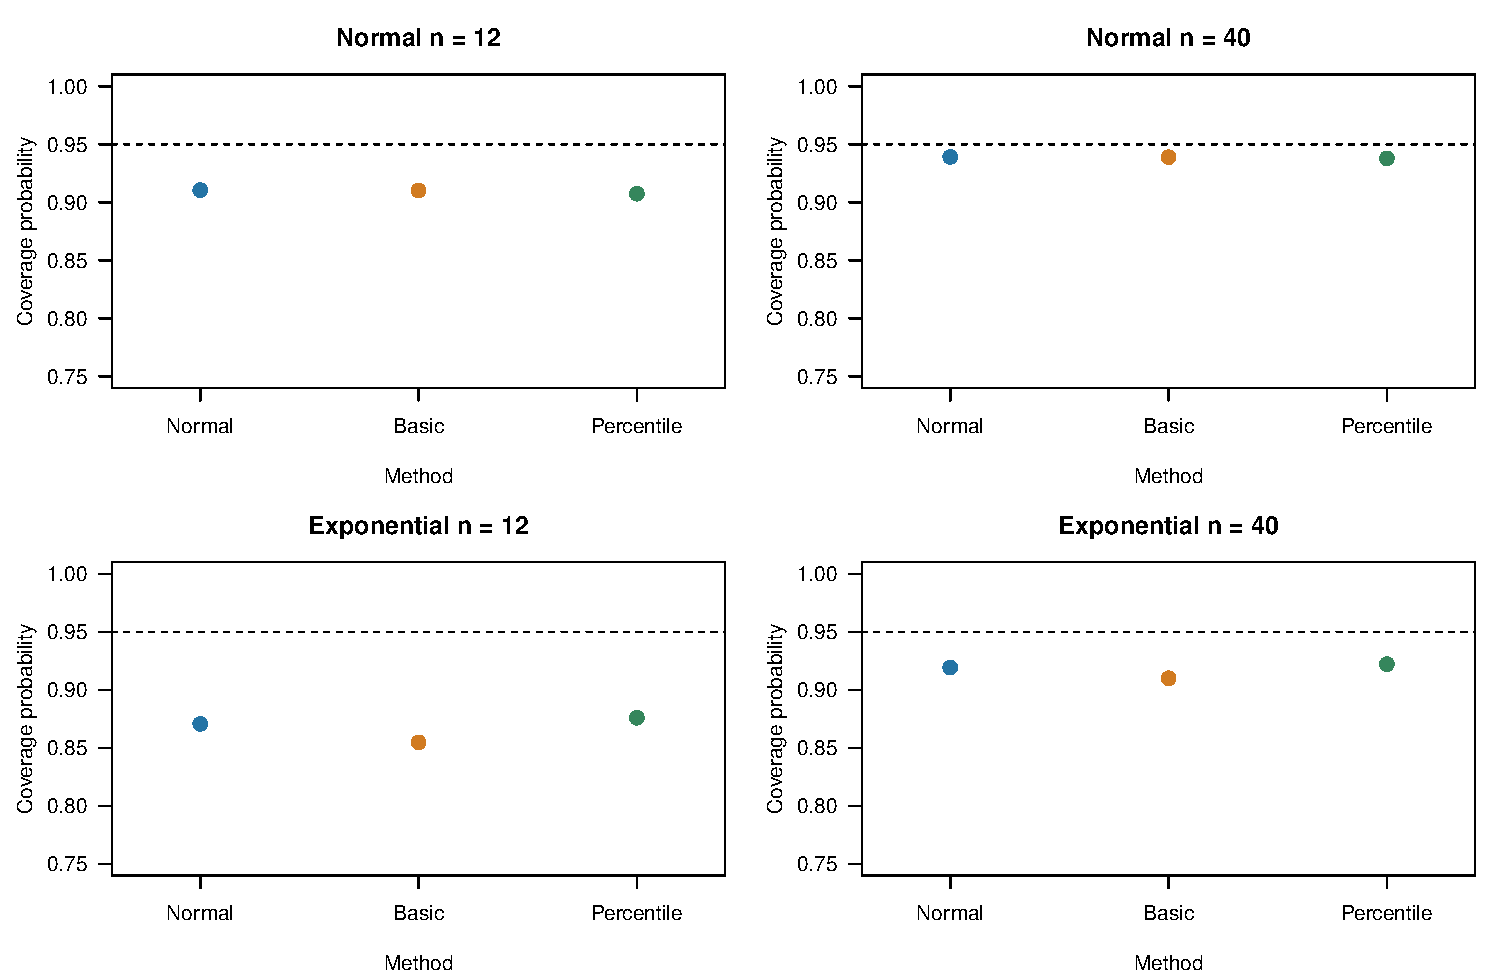
\includegraphics[width=.94\textwidth,height=.62\textheight,keepaspectratio]{assets/simulation-coverage.pdf}
\par\small Mỗi điểm là tỷ lệ bao phủ của một phương pháp. Đường ngang đứt là mức danh nghĩa 95\%.
\src{Báo cáo, hình 6.1; mã R nhóm D.}
\end{frame}
\begin{frame}{Độ dài khoảng và nhận xét}
\centering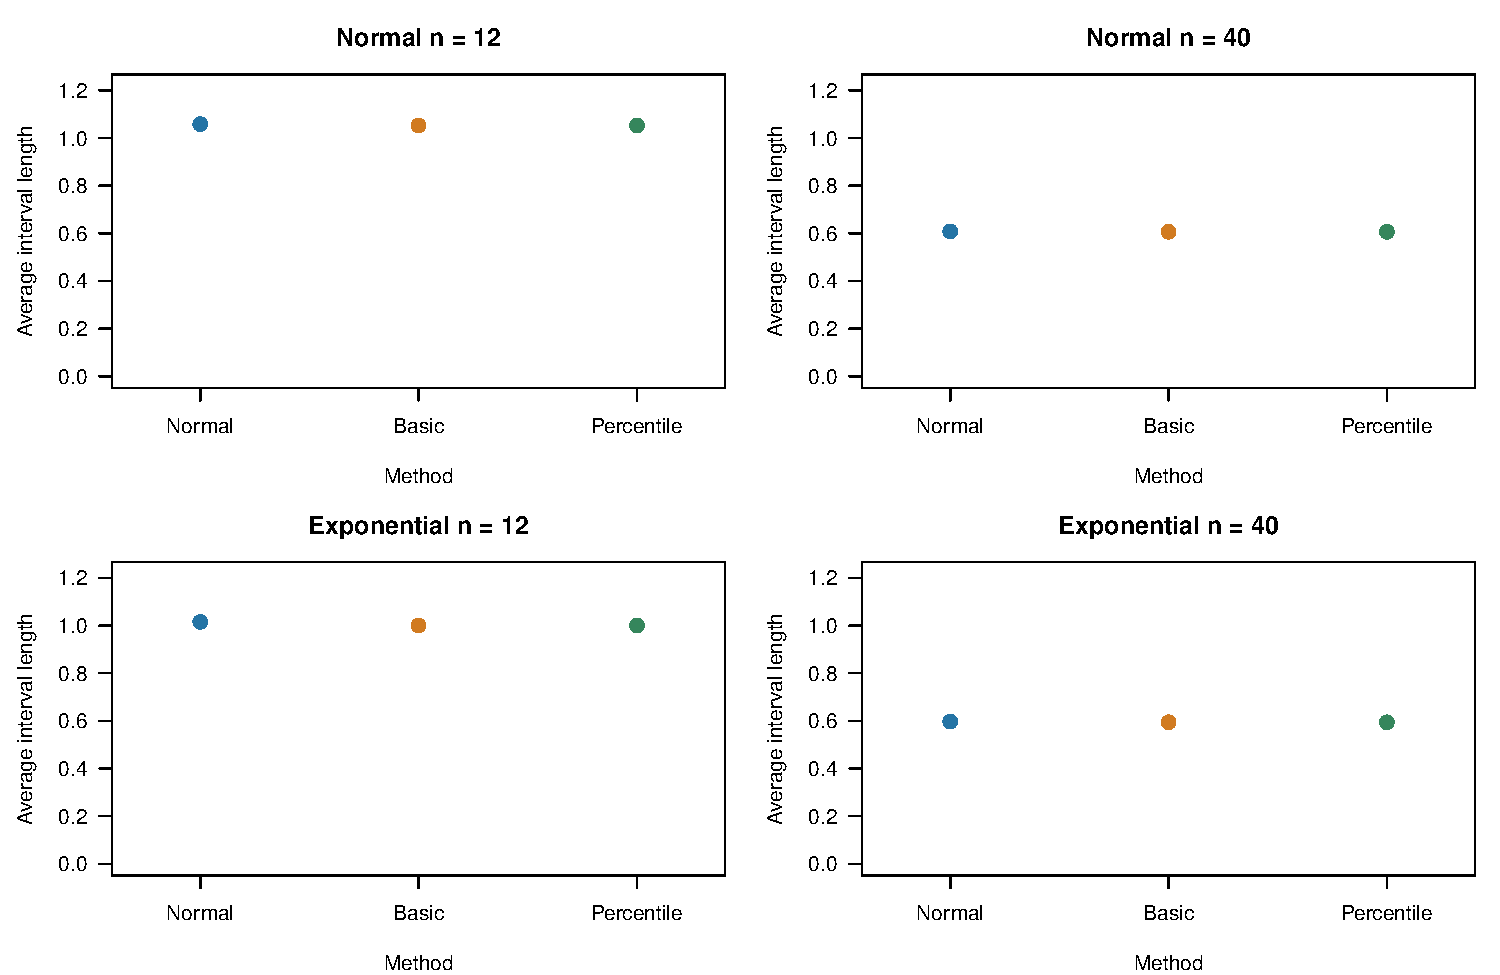
\includegraphics[width=.9\textwidth,height=.58\textheight,keepaspectratio]{assets/simulation-average-length.pdf}
\par\small Mỗi điểm là độ dài trung bình qua $K$ khoảng. Basic và Percentile dùng cùng cặp phân vị nên có cùng độ dài.
\[U_{\basic}-L_{\basic}=q_{1-\alpha/2}^*-q_{\alpha/2}^*.\]
\src{Báo cáo, hình 6.2 và nhận xét mục 6.2.}
\end{frame}
\section{Ứng dụng}
\subsection{Ví dụ và bài báo}
\begin{frame}{Ví dụ giả định: Hazard Ratio}
\small
Giả sử $\widehat{HR}=1.85$, $\sestar=0.42$, $q_{.025}^*=1.15$, $q_{.975}^*=2.82$.
\begin{align*}
CI_{\normal}&=[1.85-1.96(0.42),\;1.85+1.96(0.42)]\\
&=[1.027,2.673],\\
CI_{\basic}&=[2(1.85)-2.82,\;2(1.85)-1.15]\\
&=[0.880,2.550].
\end{align*}
\begin{itemize}
\item Normal không chứa 1, Basic chứa 1.
\item Số liệu giả định chỉ minh họa phép tính, không đánh giá coverage.
\item Với Cox, lấy lại theo bệnh nhân, giữ cùng thời gian, trạng thái và nhóm.
\end{itemize}
\src{Báo cáo, mục 7.1--7.2.}
\par\small\hyperlink{r5}{\textit{Mã Cox phân tầng trên bộ dữ liệu sinh riêng (R5)}}
\end{frame}
\begin{frame}{Bài báo: Deng và cộng sự (2013)}
\small
\textit{Using the bootstrap to establish statistical significance for relative validity comparisons among patient-reported outcome measures.}
\begin{itemize}
\item Dữ liệu: 453 bệnh nhân bệnh thận mạn, 16 thang đo.
\item Đại lượng: $RV=F_{\text{so sánh}}/F_{\text{tham chiếu}}$.
\item Bài báo chọn khoảng BCa 95\%, không phải Normal hoặc Basic.
\item Bootstrap lượng hóa độ bất định của tỷ số RV.
\end{itemize}
\begin{block}{Vai trò trong báo cáo}
Ví dụ ứng dụng Bootstrap CI thực tế. So sánh Normal--Basic được thực hiện riêng trong mô phỏng của nhóm.
\end{block}
\src{Báo cáo, mục 7.3; Deng et al. (2013), DOI: 10.1186/1477-7525-11-89.}
\end{frame}
\begin{frame}{RV và khoảng BCa được công bố}
\small\renewcommand{\arraystretch}{1.5}
\begin{tabular}{lcc}\toprule
Thang đo & RV & BCa 95\% CI\\\midrule
QDIS-CKD Static-6 &0.87&[0.72;1.03]\\
QDIS-CKD Static-34 &0.84&[0.71;0.97]\\
KDQOL Burden &0.77&[0.53;1.09]\\
KDQOL Symptoms &0.26&[0.13;0.44]\\\bottomrule
\end{tabular}
\begin{itemize}
\item Khoảng của Static-34 nằm dưới giá trị tham chiếu 1.
\item Khoảng của Burden chứa 1: RV điểm thấp hơn chưa đủ để kết luận khác biệt theo khoảng này.
\end{itemize}
\src{Báo cáo, bảng 7.1; Deng et al. (2013), bảng 1.}
\par\small\hyperlink{r4}{\textit{Vẽ lại các cận đã công bố (R4)}}
\end{frame}
\section{Mở rộng}
\subsection{Percentile và tính bất biến}
\begin{frame}{Percentile CI và quan hệ với Basic}
\begin{block}{Percentile CI}
\[CI_{\mathrm{Percentile}}=[q_{\alpha/2}^*,\;q_{1-\alpha/2}^*].\]
\end{block}
\begin{itemize}
\item Percentile lấy trực tiếp hai phân vị làm cận.
\item Basic phản chiếu hai phân vị quanh $\thn$.
\item Hai khoảng có cùng độ dài nhưng có thể khác vị trí và coverage.
\item BCa điều chỉnh các mức phân vị; báo cáo chỉ nêu như một mở rộng.
\end{itemize}
\src{Báo cáo, mục 8.1--8.3.}
\end{frame}
\begin{frame}{Bất biến của Percentile qua phép log}
Dùng cùng $B$ giá trị dương, sắp xếp thành $\hat\theta^*_{n,(r)}$.
Vì log tăng nghiêm ngặt:
\[\log\hat\theta^*_{n,(1)}\le\cdots\le\log\hat\theta^*_{n,(B)}.\]
Với type 1 và $r=\lceil Bp\rceil$:
\[q_p^*(\log\ths)=\log\hat\theta^*_{n,(r)}=\log q_p^*(\ths).\]
\begin{block}{Kết luận với cùng quy ước hạng}
Khoảng Percentile trên thang log bằng log của hai cận trên thang gốc.
\end{block}
Type 7 nội suy nên nói chung không có đẳng thức chính xác này. Basic và Normal cũng không bất biến phi tuyến nói chung.
\src{Báo cáo, mục 8.4; kiểm chứng dùng type 1. Phụ lục giải thích nội suy.}
\end{frame}

\begin{frame}{Kiểm chứng trên thang log}
\small
Mẫu $x=(2,3,4,5,9)$, cùng các bản sao và phân vị type 1.
\[\text{So sánh }\log(CI_\theta)\text{ với }CI_{\log\theta}\text{ tính lại trực tiếp}.\]
\centering\renewcommand{\arraystretch}{1.5}
\begin{tabular}{lcc}\toprule
Phương pháp & Sai khác cận lớn nhất & Khớp đến $10^{-12}$\\\midrule
Normal &0.1566453&Không\\
Basic &0.3177451&Không\\
Percentile &0&Có\\\bottomrule
\end{tabular}
\par\medskip\raggedright Kết quả là kiểm chứng trên mẫu và quy ước đã chọn, không phải thứ hạng coverage của ba khoảng.
\src{Báo cáo, bảng 8.2.}
\par\small\hyperlink{r6}{\textit{Đối chiếu hai cách tính Basic trên thang log (R6)}}
\end{frame}
\section{Kết luận}
\subsection{Phạm vi kết quả}
\begin{frame}{Kết luận}
\begin{enumerate}
\item Normal dùng xấp xỉ chuẩn và Bootstrap SE; Basic dùng phân phối sai số và đảo phân vị.
\item Trong bốn kịch bản đã xét, tăng $n$ cải thiện coverage nhưng chưa đạt 95\%.
\item Không có kết luận Basic luôn tốt hơn; cần xem coverage cùng độ dài.
\item Percentile có tính bất biến qua log khi phân vị tính bằng quy tắc hạng tương thích.
\end{enumerate}
\src{Báo cáo, mục 9; kết luận giới hạn trong thiết kế nhóm đã xét.}
\end{frame}

\begin{frame}{Đọc kết quả theo từng kịch bản}
\begin{itemize}
\item Đối chiếu $\widehat{CP}$ với mức danh nghĩa rồi so sánh độ dài trung bình.
\item Dùng MCSE để đánh giá độ dao động của kết quả do số lần lặp $K$ hữu hạn.
\item Cố định $n$ và $B$ khi so sánh các phương pháp trong cùng một kịch bản.
\item Khi đổi thang tham số, nêu rõ phép biến đổi và quy tắc phân vị.
\end{itemize}
\src{main.tex, mục 6.2, 8.4 và 9.3. Rizzo (2019), tr. 224--227.}
\end{frame}
\begin{frame}{Tài liệu tham khảo}
\scriptsize\begin{enumerate}
\item Bùi Thùy Trang (2026). \textit{Thống kê tính toán, Chương 4: Bootstrap và Jackknife.} Slide 52--60.
\item Rizzo, M. L. (2019). \textit{Statistical Computing with R}, ấn bản 2. Chapman \& Hall/CRC. Mục 6.2.1, 8.1, 8.3, 8.4 và Project 8.A.
\item Efron, B. \& Tibshirani, R. J. (1993). \textit{An Introduction to the Bootstrap.}
\item Davison, A. C. \& Hinkley, D. V. (1997). \textit{Bootstrap Methods and their Application.}
\item Bickel, P. J. \& Freedman, D. A. (1981). Some Asymptotic Theory for the Bootstrap. \textit{Annals of Statistics}, 9(6), 1196--1217.
\item Deng et al. (2013). Using the bootstrap to establish statistical significance for relative validity comparisons among patient-reported outcome measures. \textit{Health and Quality of Life Outcomes}, 11, 89. DOI: 10.1186/1477-7525-11-89.
\end{enumerate}
\src{Danh mục tài liệu tham khảo của báo cáo Nhóm D.}
\end{frame}
\appendix
\section{Phụ lục bảo vệ}
\subsection{Chứng minh và câu hỏi bổ sung}
\begin{frame}{P1. Độc lập khi giữ cố định mẫu}
Chọn $J_1,\ldots,J_n$ độc lập đều trên $\{1,\ldots,n\}$.
Với $X_i^*=x_{J_i}$ và các tập $A_i$:
\[
P^*\left(\bigcap_i\{X_i^*\in A_i\}\right)
=\prod_i\frac{\#\{j:x_j\in A_i\}}n.
\]
Đây là độc lập \emph{có điều kiện theo mẫu gốc}. Nếu không điều kiện, các bản sao cùng phụ thuộc mẫu ngẫu nhiên ban đầu.
\begin{block}{Không hoàn lại}
Lấy đủ $n$ vị trí chỉ tạo hoán vị, nên trung bình Bootstrap luôn bằng $\bar x$, không tái hiện được dao động cần đo.
\end{block}
\src{Chứng minh bổ sung từ công thức trong báo cáo Nhóm D.}
\end{frame}

\begin{frame}{P2. Vì sao mẫu số của SE là $B-1$?}
Đặt $T_b=\hat\theta_n^{*(b)}$, $m^*=E^*T_b$, $v^*=\Var^*T_b$.
\[\sum_b(T_b-\bar T)^2=\sum_b(T_b-m^*)^2-B(\bar T-m^*)^2.\]
Lấy kỳ vọng có điều kiện:
\[E^*\sum_b(T_b-\bar T)^2=Bv^*-B\frac{v^*}{B}=(B-1)v^*.\]
Chia cho $B-1$ cho phương sai không chệch. Lấy căn không bảo đảm SE không chệch.
\[se^*(\bar T)=\sqrt{v^*/B}\quad\hbox{khác}\quad se^*(T_b)=\sqrt{v^*}.\]
\src{Chứng minh bổ sung từ công thức trong báo cáo Nhóm D.}
\end{frame}

\begin{frame}{P3. SE mô phỏng hội tụ về đâu?}
Với $E^*T_b^2<\infty$, luật số lớn cho
\[\bar T\to m^*,\qquad B^{-1}\sum_bT_b^2\to E^*T_b^2\quad\mathrm{a.s.}\]
Vì vậy
\[\frac1{B-1}\sum_b(T_b-\bar T)^2
=\frac B{B-1}\left(\frac1B\sum_b T_b^2-\bar T^2\right)\to v^*.\]
Liên tục của căn trên $[0,\infty)$ cho $\sestar\to\sqrt{v^*}$.
Đây là hội tụ theo $B$, giữ cố định $x$, không phải chứng minh tính đúng của Bootstrap theo $n$.
\src{Chứng minh bổ sung từ công thức trong báo cáo Nhóm D.}
\end{frame}

\begin{frame}{P4. ECDF: hội tụ điểm và hội tụ đều}
Với mỗi $t$ cố định, luật số lớn áp dụng cho $\mathrm{I}_{\{X_i\le t\}}$:
\[F_n^*(t)\to F(t)\quad\mathrm{a.s.}\]
Định lý Glivenko--Cantelli cho mẫu i.i.d. phát biểu mạnh hơn:
\[\sup_t|F_n^*(t)-F(t)|\to0\quad\mathrm{a.s.}\]
Không được suy hội tụ đều chỉ từ hội tụ điểm.
Để suy ra độ đúng của CI còn cần tính hợp lệ của phân phối sai số Bootstrap và tính ổn định của phân vị.
\src{Báo cáo, mục 2.1; kết quả định lý được viện dẫn, không thay bằng chứng minh hội tụ điểm.}
\end{frame}

\begin{frame}{P5. Normal CI: điều kiện tiệm cận}
Giả sử $se_n>0$ và khi $n\to\infty$:
\[\frac{\thn-\theta}{se_n}\Rightarrow N(0,1),\qquad
\frac{\sestar(\thn)}{se_n}\xrightarrow{P}1.\]
Theo Slutsky:
\[\frac{\thn-\theta}{\sestar(\thn)}\Rightarrow N(0,1).\]
Suy ra $P\{\thn-z\sestar\le\theta\le\thn+z\sestar\}\to1-\alpha$.
Điều kiện này nói rõ điều cần có; nó không đúng tự động với mọi thống kê hoặc mọi $F$.
\src{Chứng minh bổ sung từ công thức trong báo cáo Nhóm D.}
\end{frame}

\begin{frame}{P6. Khi nào Basic có coverage tiệm cận?}
Đặt $a_n>0$ là thang chuẩn hóa. Giả sử
\[a_n(\thn-\theta)\Rightarrow H,\]
và phân phối có điều kiện của $a_n(\ths-\thn)$ hội tụ tới $H$ (theo xác suất), với phân vị ổn định và $H$ liên tục tại các cận.
Khi đó các phân vị sai số ước lượng hội tụ về hai phân vị của $H$. Dùng Slutsky và đảo bất đẳng thức cho
\[P\{\theta\in CI_{\basic}\}\to1-\alpha.\]
Số lần lấy lại cũng phải đủ để sai số tính phân vị không chi phối. Với trung bình thường $a_n=\sqrt n$.
\src{Chứng minh bổ sung từ công thức trong báo cáo Nhóm D.}
\end{frame}

\begin{frame}{P7. Phân vị rời rạc không kẹp đúng 95\%}
Định nghĩa $q_p=\inf\{t:G(t)\ge p\}$ cho
\[G(q_p)\ge p,\qquad G(q_p^-)\le p.\]
Với cận đóng:
\[P(q_{\alpha/2}\le T\le q_{1-\alpha/2})
=G(q_{1-\alpha/2})-G(q_{\alpha/2}^- )\ge1-\alpha.\]
Ở ví dụ lệch, $[1,7]$ chứa $255/256$. Đây là khối xác suất Bootstrap có điều kiện, không bảo đảm Basic bao phủ tham số thật ít nhất 95\%.
\src{Chứng minh bổ sung từ công thức trong báo cáo Nhóm D.}
\end{frame}

\begin{frame}{P8. Type 1 và type 7}
Với $T_{(1)}\le\cdots\le T_{(B)}$:
\begin{align*}
q_p^{*(1)}&=T_{(\lceil Bp\rceil)},\\
h&=1+(B-1)p,\quad j=\lfloor h\rfloor,\quad\gamma=h-j,\\
q_p^{*(7)}&=(1-\gamma)T_{(j)}+\gamma T_{(j+1)}.
\end{align*}
Nếu $j=B$, lấy $T_{(B)}$.
Type 1 bám ECDF, type 7 nội suy. Cả hai là quy ước hợp lệ; phải nói rõ để tái lập phép tính và tính bất biến. Hoán vị trước sắp xếp không thay kết quả.
\src{Báo cáo, mục 6.1 và 8.4; tài liệu R về quantile.}
\end{frame}

\begin{frame}{P9. SE của trung bình: tính chính xác}
Giữ cố định $x$, các $X_i^*$ độc lập cùng phân phối $F_n^*$:
\[\Var^*(\bar X^*)=\frac1{n^2}\sum_{i=1}^n\Var^*(X_i^*)
=\frac1{n^2}\sum_{j=1}^n(x_j-\bar x)^2.\]
Vì $S^2=\sum_j(x_j-\bar x)^2/(n-1)$:
\[se^*(\bar X)=\sqrt{\frac{n-1}{n}}\frac{S}{\sqrt n}.\]
Liệt kê toàn bộ $n^n$ bộ chỉ số tính moment của phân phối đã biết: dùng mẫu số $n^n$, không phải $n^n-1$.
\src{Chứng minh bổ sung từ công thức trong báo cáo Nhóm D.}
\end{frame}

\begin{frame}{P10. Vì sao chuẩn vẫn thiếu bao phủ?}
Nếu $X_i\sim N(\theta,\sigma^2)$, $\sigma>0$ và SE Bootstrap tính chính xác:
\[\theta\in CI_{\normal}\Longleftrightarrow
\left|\frac{\bar X-\theta}{S/\sqrt n}\right|\le z_{.975}\sqrt{\frac{n-1}{n}}.\]
Vế trái trong trị tuyệt đối có phân phối $t_{n-1}$. Do đó
\[CP_{\normal,\infty}=2F_{t_{n-1}}\!\left(z_{.975}\sqrt{\frac{n-1}{n}}\right)-1.\]
Khoảng 91,27\% với $n=12$; 93,98\% với $n=40$.
Đây là phép giải thích bổ sung; không phải công thức chính xác cho hữu hạn $B$ hoặc cho Basic.
\src{Chứng minh bổ sung từ công thức trong báo cáo Nhóm D.}
\end{frame}

\begin{frame}{P11. Coverage và so sánh ghép cặp}
Với $I_k=\mathrm{I}_{\{L_k\le\theta\le U_k\}}$ và $p=E(I_k)$:
\[E(\widehat{CP})=p,\quad\Var(\widehat{CP})=p(1-p)/K.\]
Thay $p$ bằng $\widehat{CP}$ để ước lượng MCSE.
So sánh cùng mẫu gốc: $D_k=I_{N,k}-I_{B,k}$:
\[\widehat\Delta=\bar D,\qquad \widehat{MCSE}(\widehat\Delta)=S_D/\sqrt K.\]
\[\Var(D_k)=\Var(I_{N,k})+\Var(I_{B,k})-2\Cov(I_{N,k},I_{B,k}).\]
Không áp dụng công thức hai tỷ lệ độc lập cho thiết kế ghép cặp.
\src{Chứng minh bổ sung từ công thức trong báo cáo Nhóm D.}
\end{frame}

\begin{frame}{P12. Log và quy tắc nội suy}
Với type 1, log giữ nguyên hạng nên bảo toàn phân vị tính từ cùng replicates dương.
Type 7 lấy trung bình có trọng số; log không giao hoán với phép lấy trung bình:
\[\log[(1-\gamma)a+\gamma b]\ne(1-\gamma)\log a+\gamma\log b.\]
Ví dụ $T=(1,4)$, $p=0{,}25$, type 7 cho
\[\log q_p(T)=\log(1{,}75)=0{,}559616,\quad q_p(\log T)=0{,}346574.\]
Với Basic: $\log(2t-q)\ne2\log t-\log q$ nói chung; phải kiểm tra các cận dương trước khi lấy log.
\src{Chứng minh bổ sung từ công thức trong báo cáo Nhóm D.}
\end{frame}

\begin{frame}{P13. Phản ví dụ cho suy luận chỉ dựa ECDF}
Giả sử $X_i\sim U(0,1)$, dùng $M_n=\max_i X_i$ ước lượng đầu mút 1.
Mọi mẫu Bootstrap đều có $M_n^*\le M_n<1$ gần chắc chắn.
\begin{block}{Hệ quả cho Percentile}
Mọi cận trên Percentile đều không vượt $M_n$, nên không chứa đầu mút thật 1: coverage bằng 0.
\end{block}
Dù ECDF vẫn hội tụ đều về $F$, hàm đầu mút và cơ chế sai số không đủ đều đặn để suy ra Bootstrap thông thường hợp lệ.
Đây là phản ví dụ bảo vệ giới hạn của khái niệm, không mở rộng mô phỏng chính của nhóm.
\src{Chứng minh bổ sung từ công thức trong báo cáo Nhóm D.}
\end{frame}

\begin{frame}{P14. Cận âm và miền tham số}
Nếu biết $\theta\in\Theta$, có thể báo tập $CI\cap\Theta$.
\[\{\theta\in CI\cap\Theta\}=\{\theta\in CI\}\quad(\theta\in\Theta).\]
Vì vậy phép giao đúng với miền đã biết không tự sửa thiếu bao phủ.
Nếu khoảng nằm hoàn toàn ngoài miền, giao có thể rỗng; không tự ép thành một điểm rồi coi là cùng thủ tục.
Các khoảng Normal/Basic có cận âm không phải lỗi trừ số; đó có thể là hạn chế của phương pháp trên thang gốc.
\src{Chứng minh bổ sung từ công thức trong báo cáo Nhóm D.}
\end{frame}
\section{Mã R trong báo cáo}

\subsection{Sáu đoạn mã nguồn}

\begin{frame}[fragile,label=r1]{R1. Mô phỏng ECDF (1/2)}
\small Sinh mẫu chuẩn, vẽ ECDF và so với CDF lý thuyết.
\begin{lstlisting}[basicstyle=\scriptsize\ttfamily]
# 1. Thiet lap tham so va phan phoi tong the N(0, 1)
set.seed(2026)
n_sizes <- c(10, 30, 100, 1000)
colors  <- c("red", "orange", "blue", "green3")

# 2. Ve CDF ly thiet
curve(pnorm(x), from = -3, to = 3, col = "black", lwd = 3, lty = 1,
main = "Minh hoa Dinh ly Glivenko-Cantelli (Hoi tu ECDF -> CDF)",
xlab = "t", ylab = "F(t)")

# 3. Ve ECDF cho cac kich thuoc mau n khac nhau
for (i in 1:length(n_sizes)) {
	n <- n_sizes[i]
	sample_data <- rnorm(n)
	fn <- ecdf(sample_data)
\end{lstlisting}
\end{frame}

\begin{frame}[fragile]{R1. Mô phỏng ECDF (2/2)}
\begin{lstlisting}[basicstyle=\scriptsize\ttfamily]
	plot(fn, add = TRUE, col = colors[i], lwd = 2, do.points = FALSE)
}

legend("topleft",
legend = c("CDF Ly thiet N(0,1)", "n = 10", "n = 30", "n = 100", "n = 1000"),
col = c("black", colors), lty = 1, lwd = 2)
\end{lstlisting}
\end{frame}

\begin{frame}[fragile,label=r2]{R2. Liệt kê mẫu đối xứng (1/1)}
\small Mỗi hàng là một bộ chỉ số. Tần số chia cho số bộ cho xác suất.
\begin{lstlisting}[basicstyle=\scriptsize\ttfamily]
x <- c(1, 2, 3)
n <- length(x)
indices <- as.matrix(do.call(expand.grid,
  c(rep(list(seq_len(n)), n), KEEP.OUT.ATTRS = FALSE)))
means <- rowMeans(matrix(x[indices], ncol = n))
support <- sort(unique(means))
frequency <- tabulate(match(means, support), length(support))
probability <- frequency / length(means)
q <- quantile(means, c(0.025, 0.975), type = 1)
\end{lstlisting}
\end{frame}

\begin{frame}[fragile,label=r3]{R3. Dựng khoảng trên một mẫu (1/1)}
\small Đoạn này dùng $x,n,B,\alpha$, \texttt{theta\_hat} và \texttt{z} từ vòng ngoài.
\begin{lstlisting}[basicstyle=\scriptsize\ttfamily]
means <- colMeans(matrix(
  x[sample.int(n, n * B, replace = TRUE)], nrow = n))
se <- sd(means)
q <- quantile(means, c(alpha / 2, 1 - alpha / 2), type = 7)
ci <- rbind(
  Normal = c(theta_hat - z * se, theta_hat + z * se),
  Basic = c(2 * theta_hat - q[2], 2 * theta_hat - q[1]),
  Percentile = q
)
\end{lstlisting}
\end{frame}

\begin{frame}[fragile,label=r4]{R4. Vẽ lại khoảng BCa (1/3)}
\small Mã sử dụng các cận BCa đã công bố để vẽ lại biểu đồ.
\begin{lstlisting}[basicstyle=\scriptsize\ttfamily]
measure <- c(
"KDQOL Symptoms",
"KDQOL Burden",
"QDIS-CKD Static-34",
"QDIS-CKD Static-6"
)

rv <- c(0.26, 0.77, 0.84, 0.87)
lower <- c(0.13, 0.53, 0.71, 0.72)
upper <- c(0.44, 1.09, 0.97, 1.03)
y <- seq_along(rv)

png("deng_bca_ci.png", width = 1800, height = 1100, res = 200)

par(mar = c(5, 10, 3, 2))
\end{lstlisting}
\end{frame}

\begin{frame}[fragile]{R4. Vẽ lại khoảng BCa (2/3)}
\begin{lstlisting}[basicstyle=\scriptsize\ttfamily]
plot(
rv, y,
xlim = c(0, 1.2),
ylim = c(0.5, 4.5),
yaxt = "n",
ylab = "",
xlab = "Relative validity (RV) va khoang tin cay BCa 95%",
main = "Khoang BCa cua mot so cong cu trong nghien cuu Deng et al. (2013)",
pch = 19
)

axis(2, at = y, labels = measure, las = 1)
segments(lower, y, upper, y, lwd = 2)
segments(lower, y - 0.08, lower, y + 0.08, lwd = 2)
segments(upper, y - 0.08, upper, y + 0.08, lwd = 2)
\end{lstlisting}
\end{frame}

\begin{frame}[fragile]{R4. Vẽ lại khoảng BCa (3/3)}
\begin{lstlisting}[basicstyle=\scriptsize\ttfamily]
abline(v = 1, lty = 2, col = "red", lwd = 2)

legend(
"bottomright",
legend = "RV = 1 (muc tham chieu)",
col = "red",
lty = 2,
lwd = 2,
bty = "n"
)

dev.off()
\end{lstlisting}
\end{frame}

\begin{frame}[fragile,label=r5]{R5. Bootstrap HR phân tầng (1/4)}
\small Dữ liệu được sinh với seed 2026. Khi lấy lại theo nhóm, giữ nguyên từng dòng \texttt{time, status, group}.
\begin{lstlisting}[basicstyle=\scriptsize\ttfamily]
# 1. Sinh du lieu gia dinh Thoi gian song sot va Trang thai (1: Bien co, 0: Khuyet)
set.seed(2026)
n <- 40
group <- rep(c(0, 1), each = n/2) # 0: Control, 1: Treatment
# Sinh thoi gian theo phan phoi Mu phu thuoc vao nhom
time <- rexp(n, rate = 0.1 * exp(-0.6 * group))
status <- rbinom(n, size = 1, prob = 0.85) # 85% quan sat duoc bien co

data_med <- data.frame(time = time, status = status, group = group)

# 2. Tinh Hazard Ratio (HR) tren mau goc qua mo hinh Cox
library(survival)
fit_orig <- coxph(Surv(time, status) ~ group, data = data_med)
hr_hat <- exp(coef(fit_orig))

\end{lstlisting}
\end{frame}

\begin{frame}[fragile]{R5. Bootstrap HR phân tầng (2/4)}
\begin{lstlisting}[basicstyle=\scriptsize\ttfamily]
# 3. Stratified Bootstrap Monte Carlo (B = 2000)
B <- 2000
boot_hrs <- numeric(B)

for (b in 1:B) {
	# Rut mau phan tang theo nhom
	idx0 <- sample(which(data_med$group == 0), replace = TRUE)
	idx1 <- sample(which(data_med$group == 1), replace = TRUE)
	boot_data <- data_med[c(idx0, idx1), ]

	fit_boot <- coxph(Surv(time, status) ~ group, data = boot_data)
	boot_hrs[b] <- exp(coef(fit_boot))
}

# 4. Tinh dac trung va Khoang tin cay
\end{lstlisting}
\end{frame}

\begin{frame}[fragile]{R5. Bootstrap HR phân tầng (3/4)}
\begin{lstlisting}[basicstyle=\scriptsize\ttfamily]
se_star <- sd(boot_hrs)
q_low   <- quantile(boot_hrs, 0.025)
q_upp   <- quantile(boot_hrs, 0.975)

ci_normal <- c(hr_hat - 1.96 * se_star, hr_hat + 1.96 * se_star)
ci_basic  <- c(2 * hr_hat - q_upp, 2 * hr_hat - q_low)

cat("Original HR Hat:", round(hr_hat, 3), "\n")
cat("Normal CI (95%): [", round(ci_normal[1], 3), ",", round(ci_normal[2], 3), "]\n")
cat("Basic CI  (95%): [", round(ci_basic[1], 3), ",", round(ci_basic[2], 3), "]\n")

# 5. Ve do thi phan phoi Bootstrap HR va Khoang tin cay
hist(boot_hrs, breaks = 35, probability = TRUE, col = "aliceblue",
main = "Phan phoi Bootstrap cho Hazard Ratio (HR) trong Nghien cuu Y sinh",
xlab = "Gia tri Hazard Ratio Bootstrap (HR*)", border = "white")
\end{lstlisting}
\end{frame}

\begin{frame}[fragile]{R5. Bootstrap HR phân tầng (4/4)}
\begin{lstlisting}[basicstyle=\scriptsize\ttfamily]
lines(density(boot_hrs), col = "darkblue", lwd = 2)

# Ve duong nguong HR = 1.0 va vi tri HR Hat
abline(v = 1.0, col = "gray40", lwd = 2, lty = 3) # Nguong khong co tac dung
abline(v = hr_hat, col = "black", lwd = 2, lty = 1)

# Ve thanh Khoang tin cay Normal CI vs Basic CI
y_m <- max(density(boot_hrs)$y)
lines(ci_normal, c(y_m * 0.75, y_m * 0.75), col = "red", lwd = 4)
lines(ci_basic,  c(y_m * 0.55, y_m * 0.55), col = "green3", lwd = 4)

legend("topright",
legend = c("HR Hat", "Nguong HR=1.0", "Normal CI", "Basic CI"),
col = c("black", "gray40", "red", "green3"), lty = c(1, 3, 1, 1), lwd = c(2, 2, 4, 4))
\end{lstlisting}
\end{frame}

\begin{frame}[fragile,label=r6]{R6. Kiểm chứng Basic dưới log (1/2)}
\small Dùng cùng các bản sao ở hai thang. Đoạn trích dùng $B$ và \texttt{tail\_probs} từ mã mô phỏng.
\begin{lstlisting}[basicstyle=\scriptsize\ttfamily]
invariance_sample <- c(2, 3, 4, 5, 9)
invariance_n <- length(invariance_sample)
invariance_indices <- matrix(
  sample.int(invariance_n, invariance_n * B, replace = TRUE),
  nrow = invariance_n)
bootstrap_theta <- colMeans(matrix(
  invariance_sample[invariance_indices], nrow = invariance_n))
theta_hat <- mean(invariance_sample)
eta_hat <- log(theta_hat)
bootstrap_eta <- log(bootstrap_theta)
q_theta <- quantile(bootstrap_theta, tail_probs, type = 1)
q_eta <- quantile(bootstrap_eta, tail_probs, type = 1)
ci_theta <- c(2 * theta_hat - q_theta[2],
              2 * theta_hat - q_theta[1])
ci_eta_transformed <- log(ci_theta)
\end{lstlisting}
\end{frame}

\begin{frame}[fragile]{R6. Kiểm chứng Basic dưới log (2/2)}
\begin{lstlisting}[basicstyle=\scriptsize\ttfamily]
ci_eta_direct <- c(2 * eta_hat - q_eta[2],
                   2 * eta_hat - q_eta[1])
max_abs_difference <- max(abs(ci_eta_transformed - ci_eta_direct))
\end{lstlisting}
\end{frame}
\end{document}
